\section{Circuit Design and Operation}

This section examines the amplifier control circuit, specifically the PWM oscillator.

%TODO: discussion of operation

\subsection{Selection of Component Values}

The desired PWM oscillation frequency for the circuit is 300 Hz.
A diagram for the oscillator, taken from the instruction manual for the motor control kit, may be seen in figure 1; component numbers used henceforth refer to this diagram.
As presented during lecture, equations \ref{eq:T1} and \ref{eq:T2} show the two time components of the oscillator output, rise time and fall time.
Given the 300 Hz desired frequency, component values must be found to satisfy equation \ref{eq:desiredF}.
 
\begin{figure}[h]
    \label{fig:oscillatorcapture}
    \centering
    \includegraphics[width=.22\textwidth,bb=0 0 300 419]{images/OscillatorCapture.PNG}
    \caption{Circuit Oscillator Circuit - From Manual}
\end{figure}
 
\begin{equation}
	\label{eq:T1}
	T_1 = {\it R_5}\,C\ln  \left( {\frac {{\it R_3}\,{\it V^+}}{{\it R_4}\, \left( {
\it V^+}-{\it V_{in}} \right) }}+1 \right) 
\end{equation}

\begin{equation}
	\label{eq:T2}
	T_2 = {\it R_5}\,C\ln  \left( {\frac {{\it R_3}\,{\it V^+}}{{\it R_4}\,{\it V_{in}}}
}+1 \right) 
\end{equation}

\begin{equation}
	\label{eq:desiredF}
	300= {\frac {1}{T_1 + T_2}}
\end{equation}

There is a single constraint equation (the frequency) and four component values appearing in the equation which must be chosen.
As such, three component values must be fixed, arbitrarily or based on external constraints, to solve for the last component value which gives a 300 Hz frequency.
%
%More explanaition of the following might be needed
Resistor $R_3$ acts to scale the input voltage and therefore only impacts frequency to the extent that the input voltage does.
Similarly, resistor $R_4$ simply determines the gain of the op-amp, and offsets the output voltage. 
The values for $R_3$ and $R_4$ were set as those of the actual circuit, $47 k\Omega$ and $220 k\Omega$ respectively.
The capacitors value was also fixed at $10 nF$ and $V^{+}$ was set to 8 V, the same value used when testing the circuit.
Given these constraints, the desired value of $R_5$ for a 300 Hz frequency is shown in equation \ref{eq:R5}.

\begin{equation}
	\label{eq:R5}
	R_5 = {\frac {1000000}{3}}\, \left( \ln  \left( {\frac {1}{55}}\,{\frac {-
534+55\,{\it V_{in}}}{-8+{\it V_{in}}}} \right) +\ln  \left( {\frac {1}{55}}\,
{\frac {94+55\,{\it V_{in}}}{{\it V_{in}}}} \right)  \right) ^{-1}
\end{equation}

It can be seen from equation \ref{eq:R5} that the value of $R_5$ which produces a 300 Hz output frequency depends on the input voltage which is variable.
The relationship between input voltage and the desired value for $R_5$ is shown in figure 2.
A single $V_{in}$ must be chosen to determine the value of $R_5$. 
Using a \q{center} input voltage ($V_{in} = 2.28 V$ from figure 5), or the voltage for which the motor is disabled, the desired value for $R_5$ is  $406.1 k\Omega$.
This value is quite close to the value used on the board $470 k\Omega$.

\begin{figure}[h]
    \label{fig:VinR5}
    \centering
    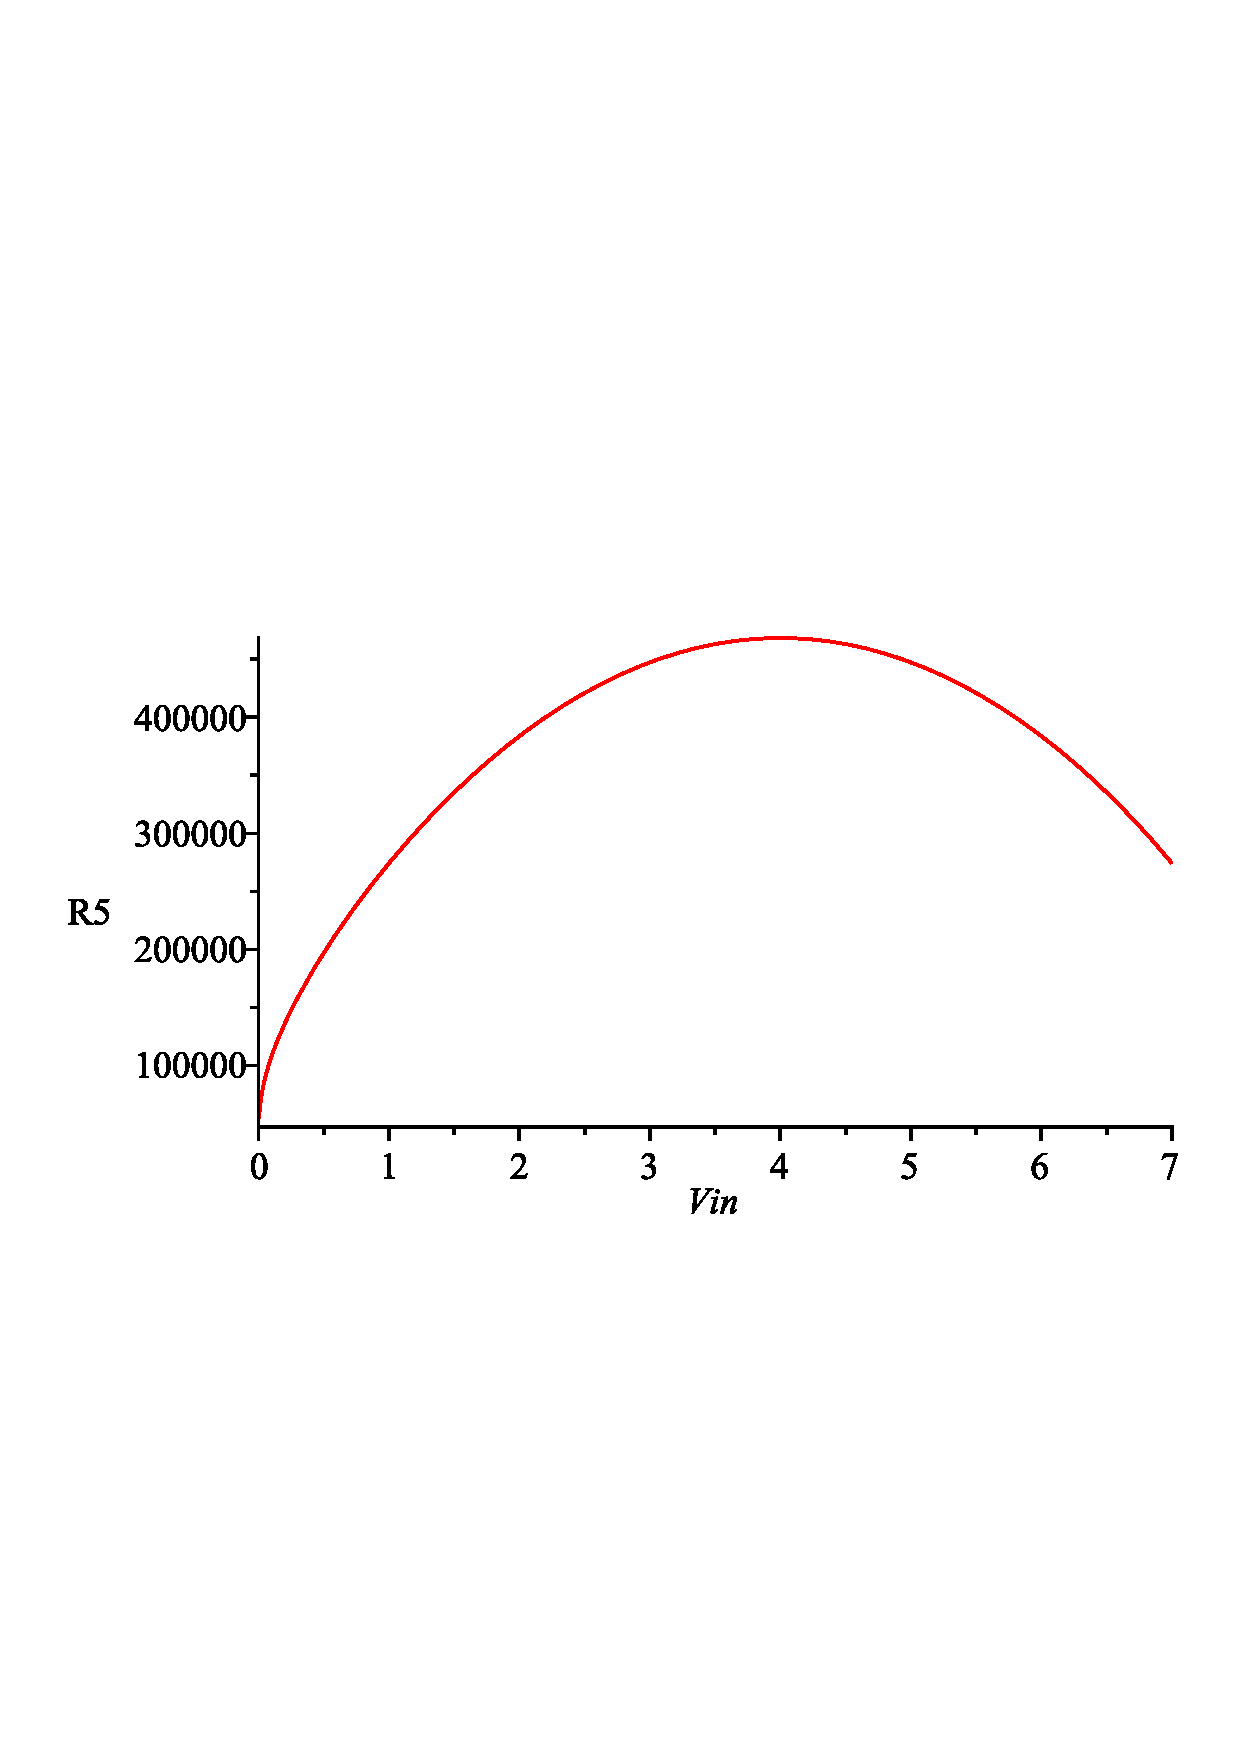
\includegraphics[width=.70\textwidth]{images/VinR5.pdf}
    \caption{Input Voltage Vs Desired Value for $R_5$ for 300 Hz Frequency}
\end{figure}

A circuit simulation confirms a nominal frequency very close to 300 Hz.
To verify the frequency, a Fourier transform of the oscillator output for $V_{in} = 2.28 V$ and $R_5 = 406.1 k\Omega$ is shown in figure 3. 
It can be seen that the dominant frequency is approximately 300 Hz.
%	TODO: Why approximately
A theoretical plot of duty cycle over a range of input voltages may be seen in figure 4.

\begin{figure}[h]
    \label{fig:FFT}
    \centering
    \includegraphics[width=.70\textwidth,bb=0 0 1056 406]{images/FFT.png}
    \caption{Fast Fourier Transform of Simulated Oscillator Output}
\end{figure}

\begin{figure}[h]
    \label{fig:dutycycle}
    \centering
    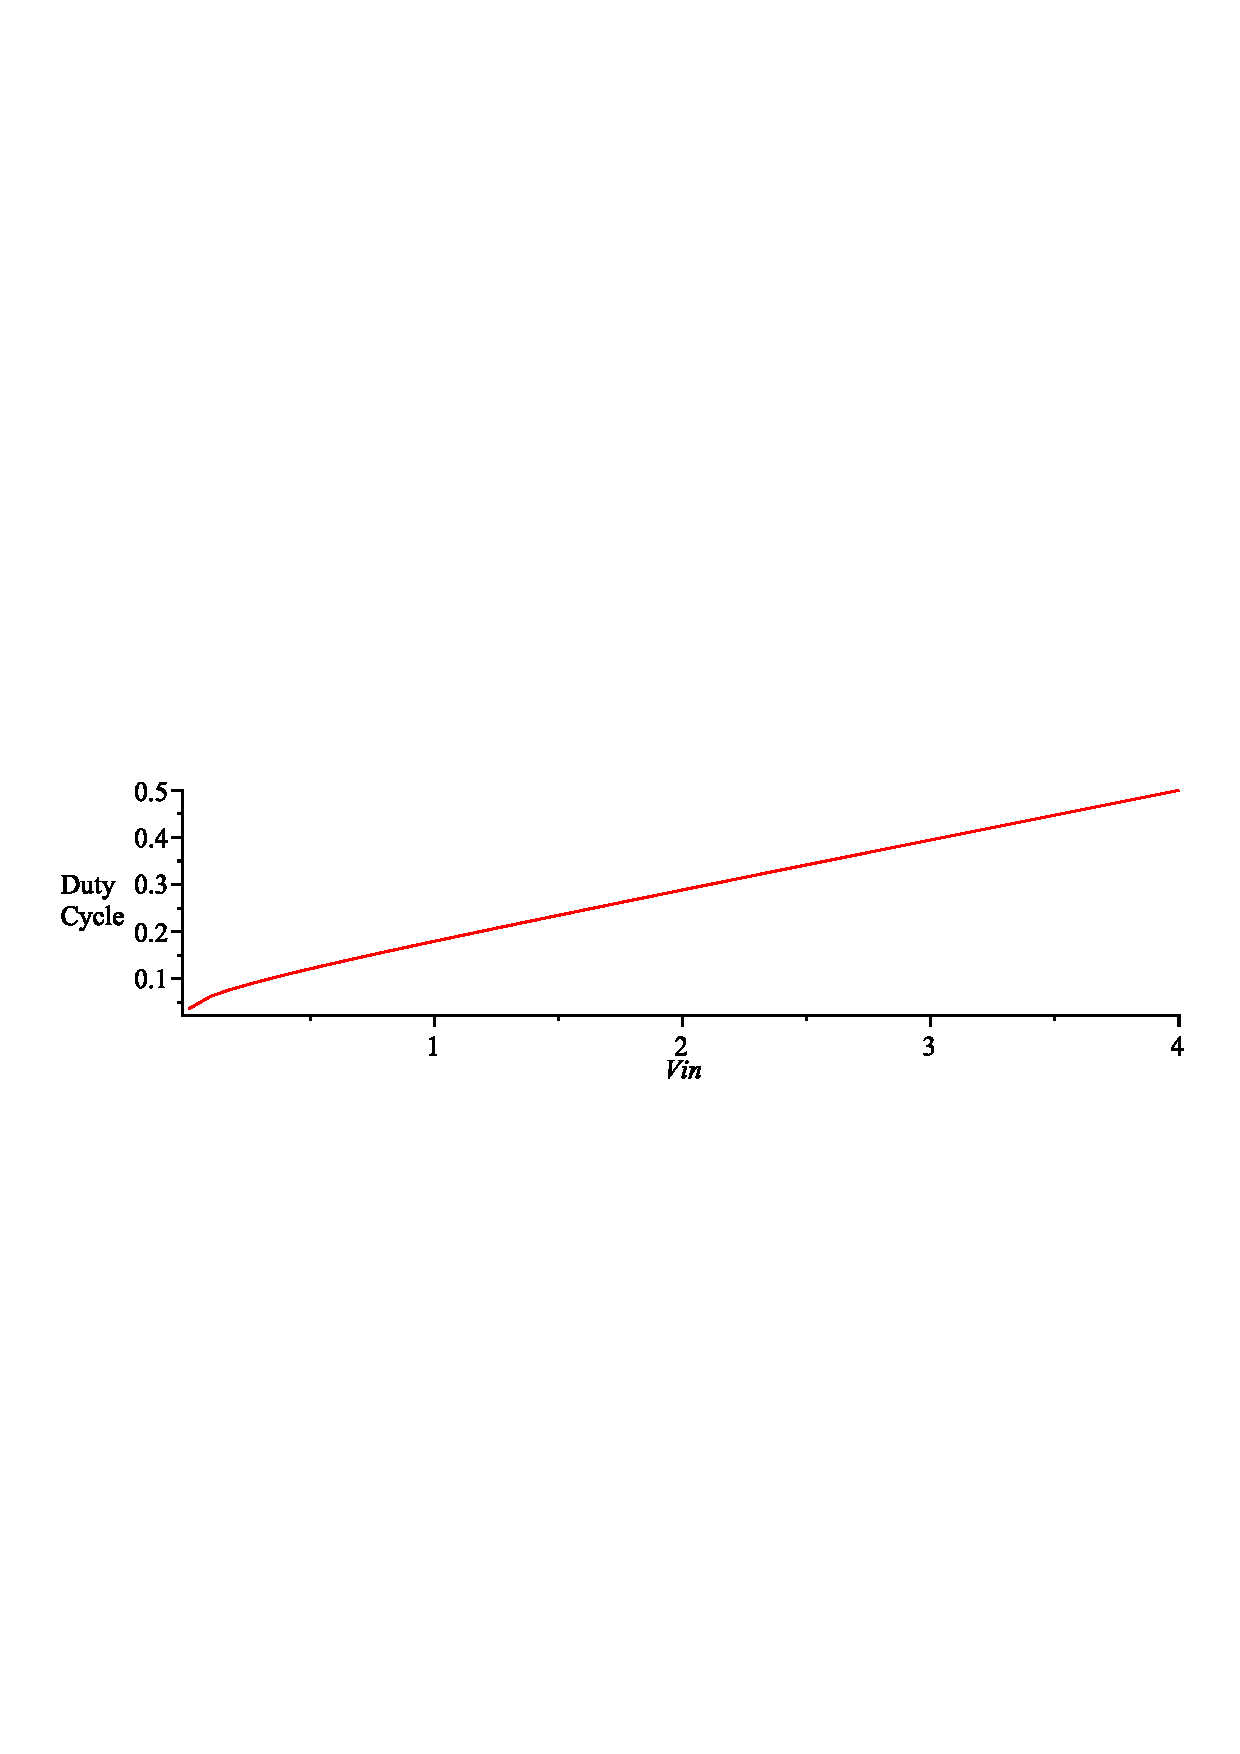
\includegraphics[width=.70\textwidth]{images/dutycycle.pdf}
    \caption{Oscillator Duty Cycle for $V_{in} = 0$ to $V_{in} = {\frac {V^+}{2}}$}
\end{figure}

\subsection{Input Output Characterization}

The input-output characteristics of the amplifier were examined for the simulated circuit and the actual circuit.
The result may be seen in figure 5.
It should be noted that the simulated circuit had no load whereas the actual circuit was driving the motor, with no load.
Sample values are given in table \ref{tbl:iovalues}.
Refer to section \ref{sec:tf} for an overview of the process used to obtain experimental values.

\begin{figure}[h]
    \label{fig:io}
    \centering
    \includegraphics[width=.70\textwidth,bb=0 0 1149 467]{images/OutputVoltage.png}
    \caption{Input-Output Characterization for Simulated (Unloaded) and Actual (Loaded with Motor) Circuit}
\end{figure}

\begin{table}[h]
	\centering
	\caption{Input-Output Characterization}
	\label{tbl:iovalues}
	\vspace{6pt}
	\footnotesize
	\begin{tabular}{ccc}
		\toprule
		$V_{in}$ & $V_{out}$ (Actual) & $V_{out}$ (Simulated) \\
		\midrule
		3.8 & 8.06 & 6.4819629 \\
		2.90 &7.8 & 2.1355862 \\
		2.799 &7.71 & 1.6661552 \\
		2.6 &7.38 & 0.7739846 \\
		2.515 &7.0 & 0.394138 \\
		2.459 &6.70 & 0.1553944 \\
		2.43 &6.48 & 0.0338252 \\
		2.4 &6.0 & 0.0016906 \\
		2.39 &5.95 & 0.0012864 \\
		2.34 &4.89 & 0.0002554 \\
		2.31 &3.77 & -0.0002944 \\
		2.29 &2.8 & -0.0008018 \\
		2.28 &2.72 & -0.001161 \\
		2.27 &1.23 & -0.001596 \\
		2.265 &1.2 & -0.0018552 \\
		2.261 &1.1 & 0.8382106 \\
		2.25 &0.81 & -0.0029108 \\
		1.81 &-1.9 & -1.7913446 \\
		1.791 &-2.75 & -1.8549068 \\
		1.752 &-4.56 & -2.1259024 \\
		1.746 &-4.92 & -2.0894574 \\
		1.709 &-5.96 & -2.2841442 \\
		1.665 &-6.64 &- 2.5689882 \\
		1.630 &-6.94 & -2.748412 \\
		1.572 &-7.27 & -3.0502118 \\
		1.555 &-7.33 & -3.1671898 \\
		1.425 &-7.64 & -3.82 \\
		0.338 &-8.04 & -7.00 \\
		\bottomrule
	\end{tabular}
\end{table}
